\section{Hierarchical Extension}

\begin{frame}{That's Not Enough\dots}

\begin{figure}

\foreach \n in {1,...,9}{%
\includegraphics<\n>[width=0.8\textwidth]{img/recursive/level-\n}%
}%

\caption{An overplayed meme in academic circles.}

\end{figure}

\end{frame}

\begin{frame}{Clumps \& Clumps of Clumps}

\vspace{4ex}

\begin{figure}
\begin{columns}
\begin{column}{0.05\textwidth}
\begin{subfigure}[b]{\textwidth}
\caption{}
\label{fig:natural}
\end{subfigure}
\end{column}
\begin{column}{0.27\textwidth}
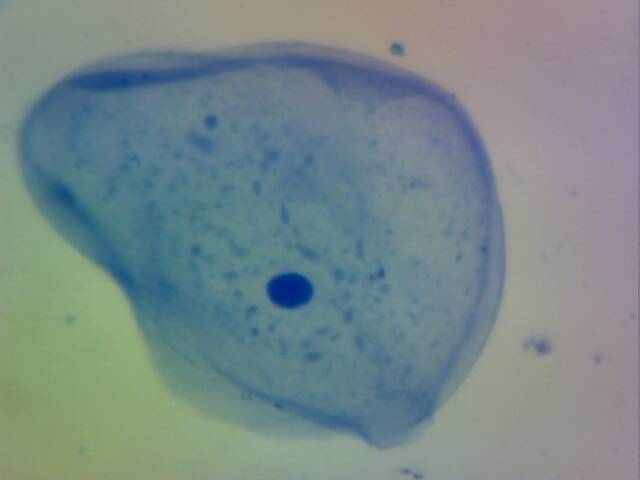
\includegraphics[width=\textwidth]{cheek_cell}
\end{column}
\begin{column}{0.07\textwidth}

\includegraphics[width=\textwidth]{arrow}
\end{column}
\begin{column}{0.27\textwidth}
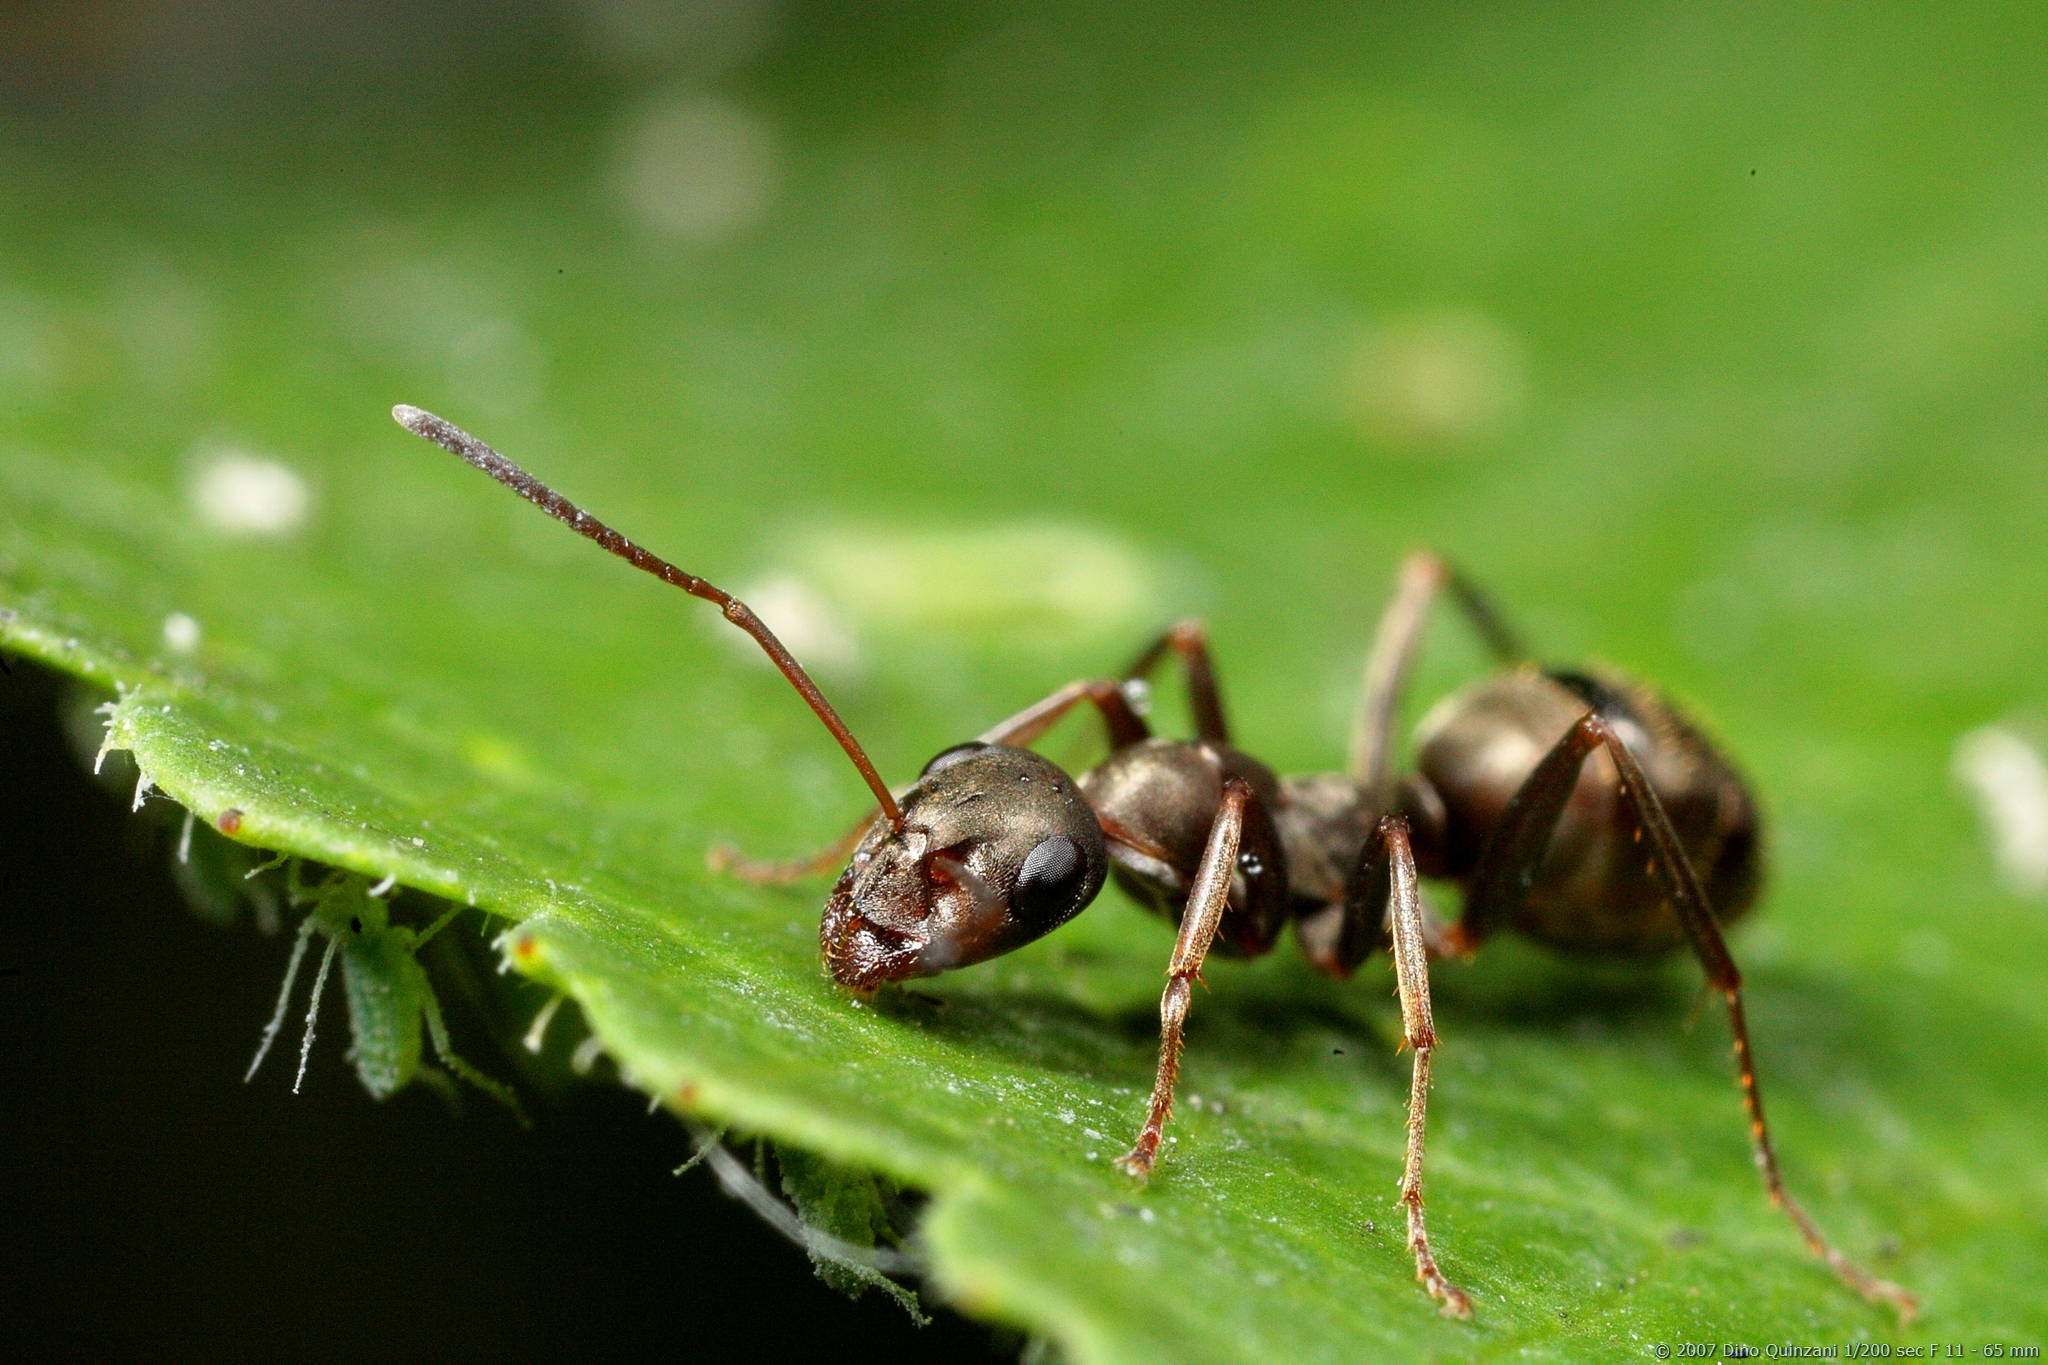
\includegraphics[width=\textwidth]{ant}
\end{column}
\begin{column}{0.07\textwidth}

\includegraphics[width=\textwidth]{arrow}
\end{column}
\begin{column}{0.27\textwidth}
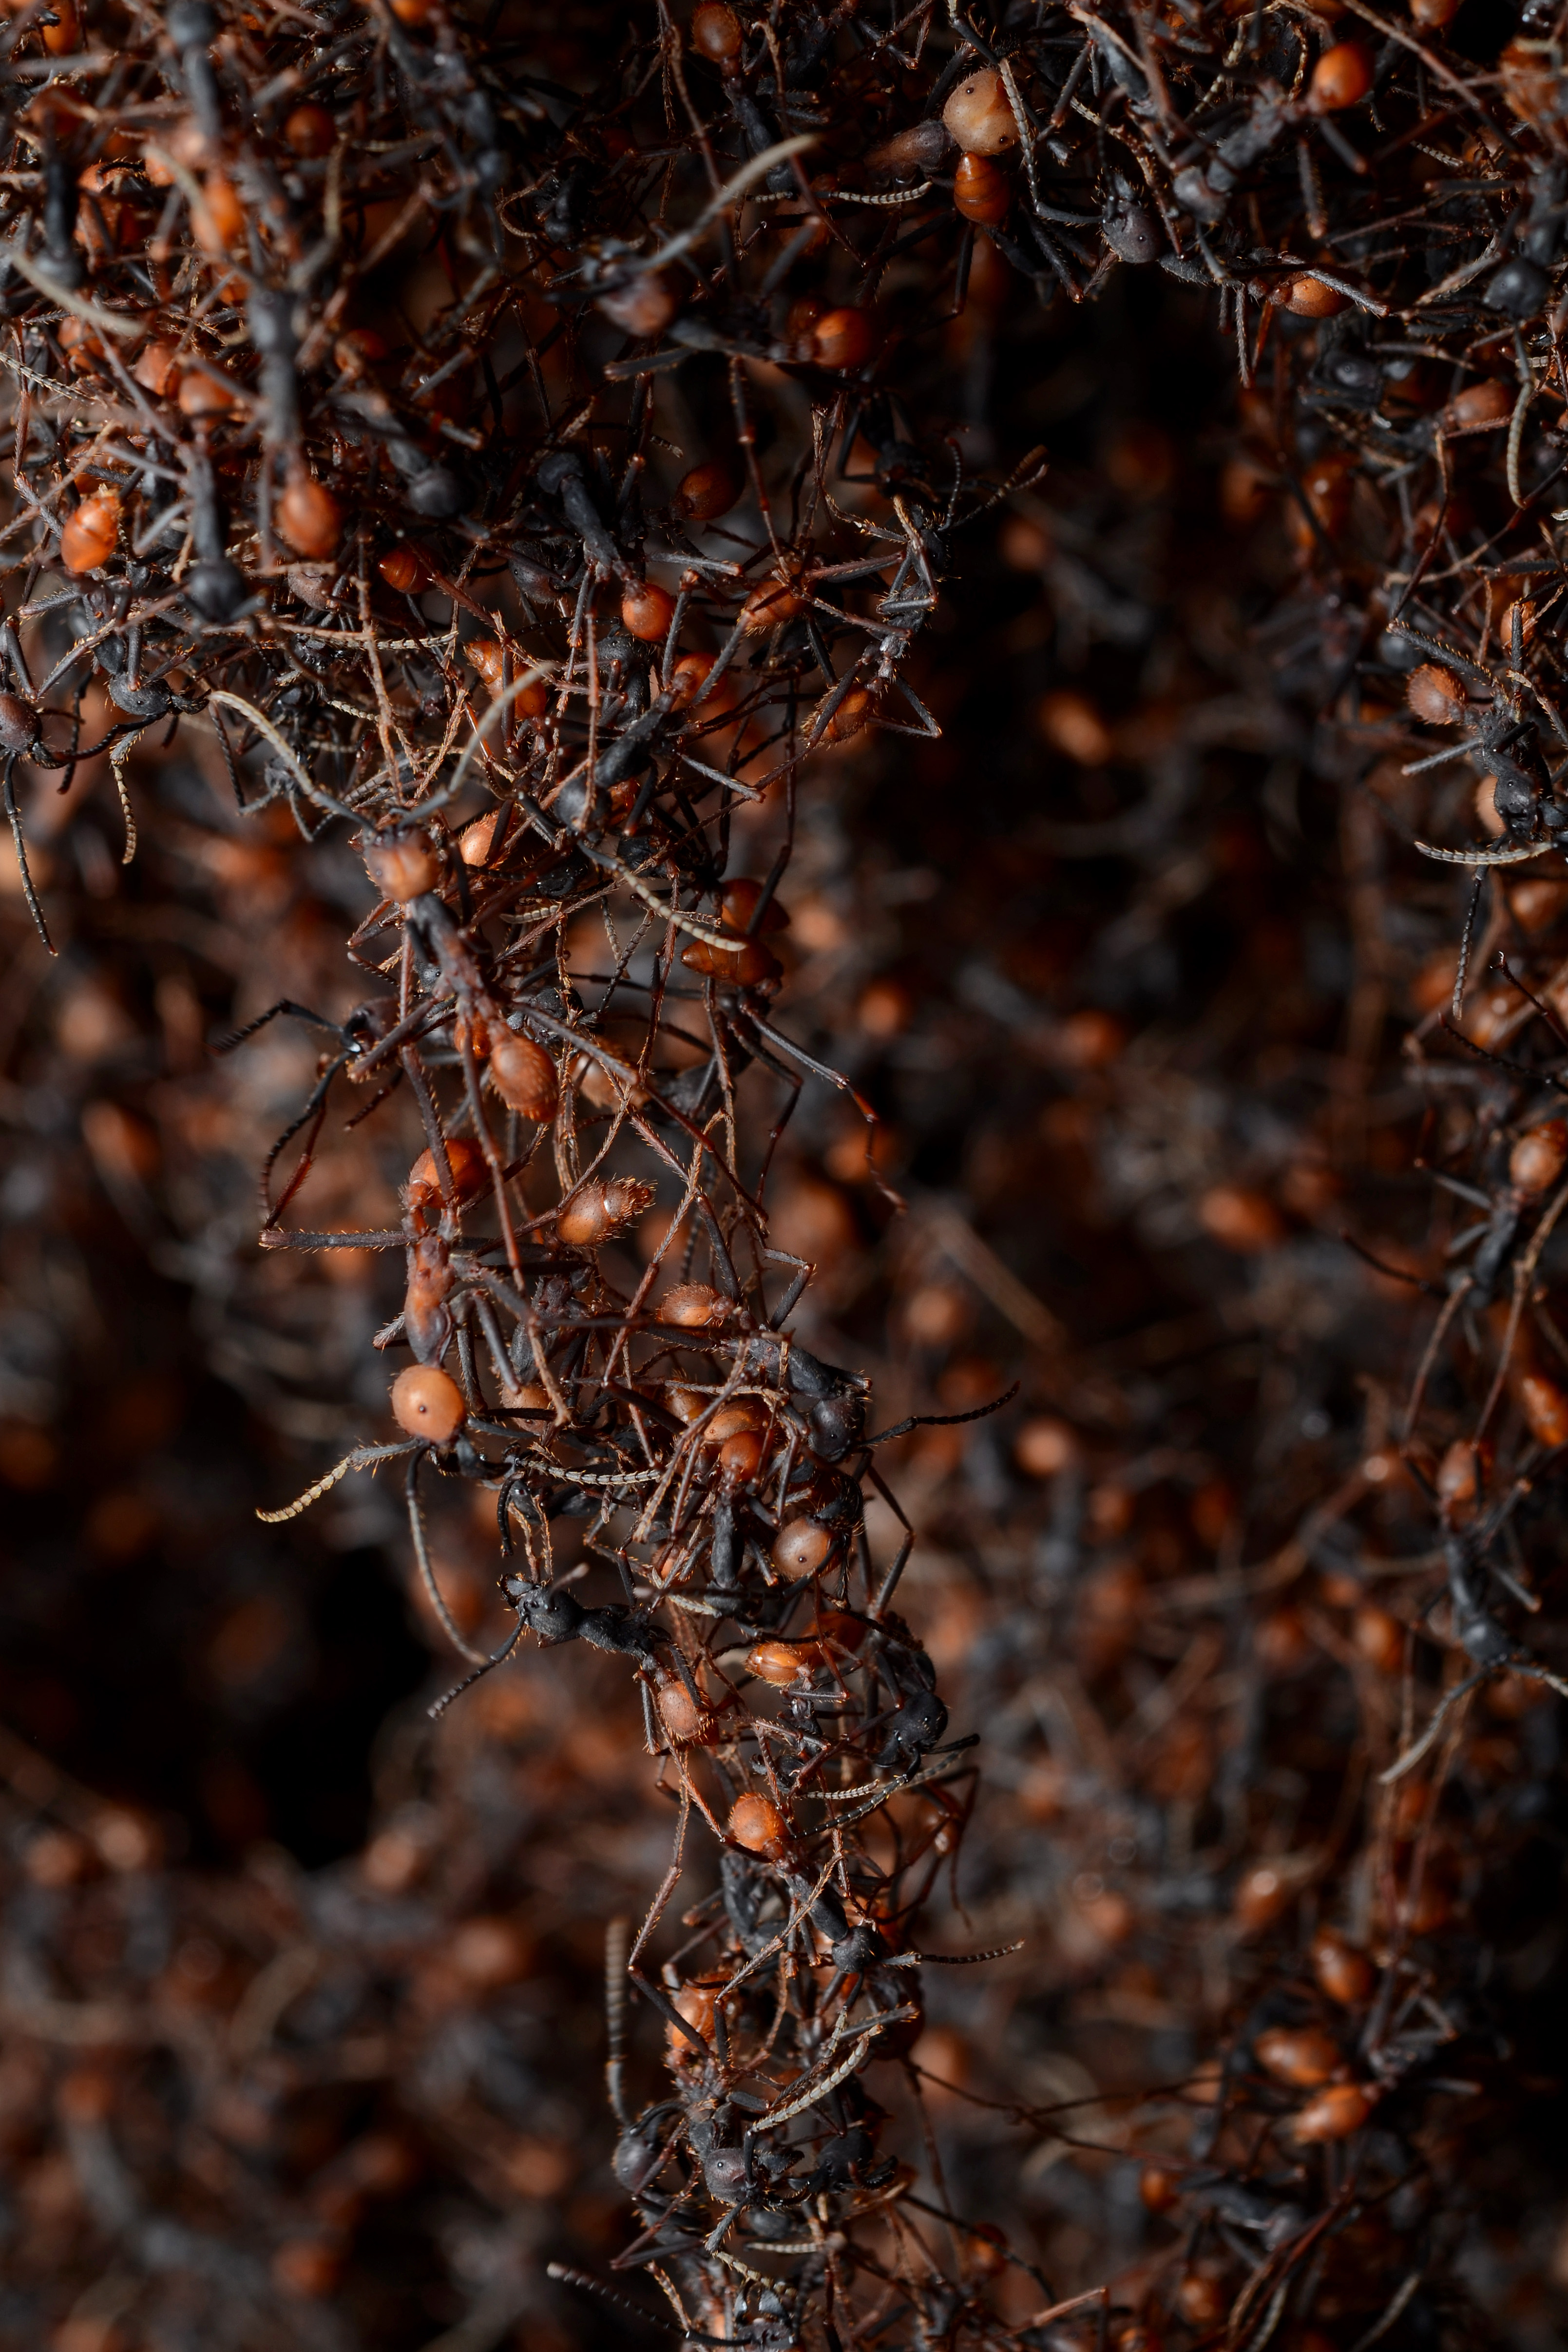
\includegraphics[angle=270, width=\textwidth]{ant_bridge}
\end{column}
\end{columns}
\vspace{1ex}
\begin{columns}
\begin{column}{0.05\textwidth}
\end{column}
\begin{column}{0.27\textwidth}
\centering
cell {\tiny\cite{clare_and_ben_2017}}
\end{column}
\begin{column}{0.07\textwidth}
\end{column}
\begin{column}{0.27\textwidth}
\centering
ant {\tiny\cite{quinzani_2008}}
\end{column}
\begin{column}{0.07\textwidth}
\end{column}
\begin{column}{0.27\textwidth}
\centering
ant colony {\tiny\cite{gallice_2011}}
\end{column}
\end{columns}
\begin{columns}
\begin{column}{0.05\textwidth}
\end{column}
\begin{column}{0.27\textwidth}
\centering
\end{column}
\begin{column}{0.07\textwidth}
\end{column}
\begin{column}{0.27\textwidth}
\centering
(clump)
\end{column}
\begin{column}{0.07\textwidth}
\end{column}
\begin{column}{0.27\textwidth}
\centering
(clump of clumps)
\end{column}
\end{columns}
\vspace{2ex}
\begin{columns}
\begin{column}{0.05\textwidth}
\begin{subfigure}[b]{\textwidth}
\caption{}
\label{fig:simulated}
\end{subfigure}
\end{column}
\begin{column}{0.27\textwidth}

\includegraphics[width=\textwidth]{cell}
\end{column}
\begin{column}{0.07\textwidth}
{\Large$\underset{\phantom{\checkmark}}{\overset{\checkmark}{
\includegraphics[width=\textwidth]{arrow}}}$}
\end{column}
\begin{column}{0.27\textwidth}
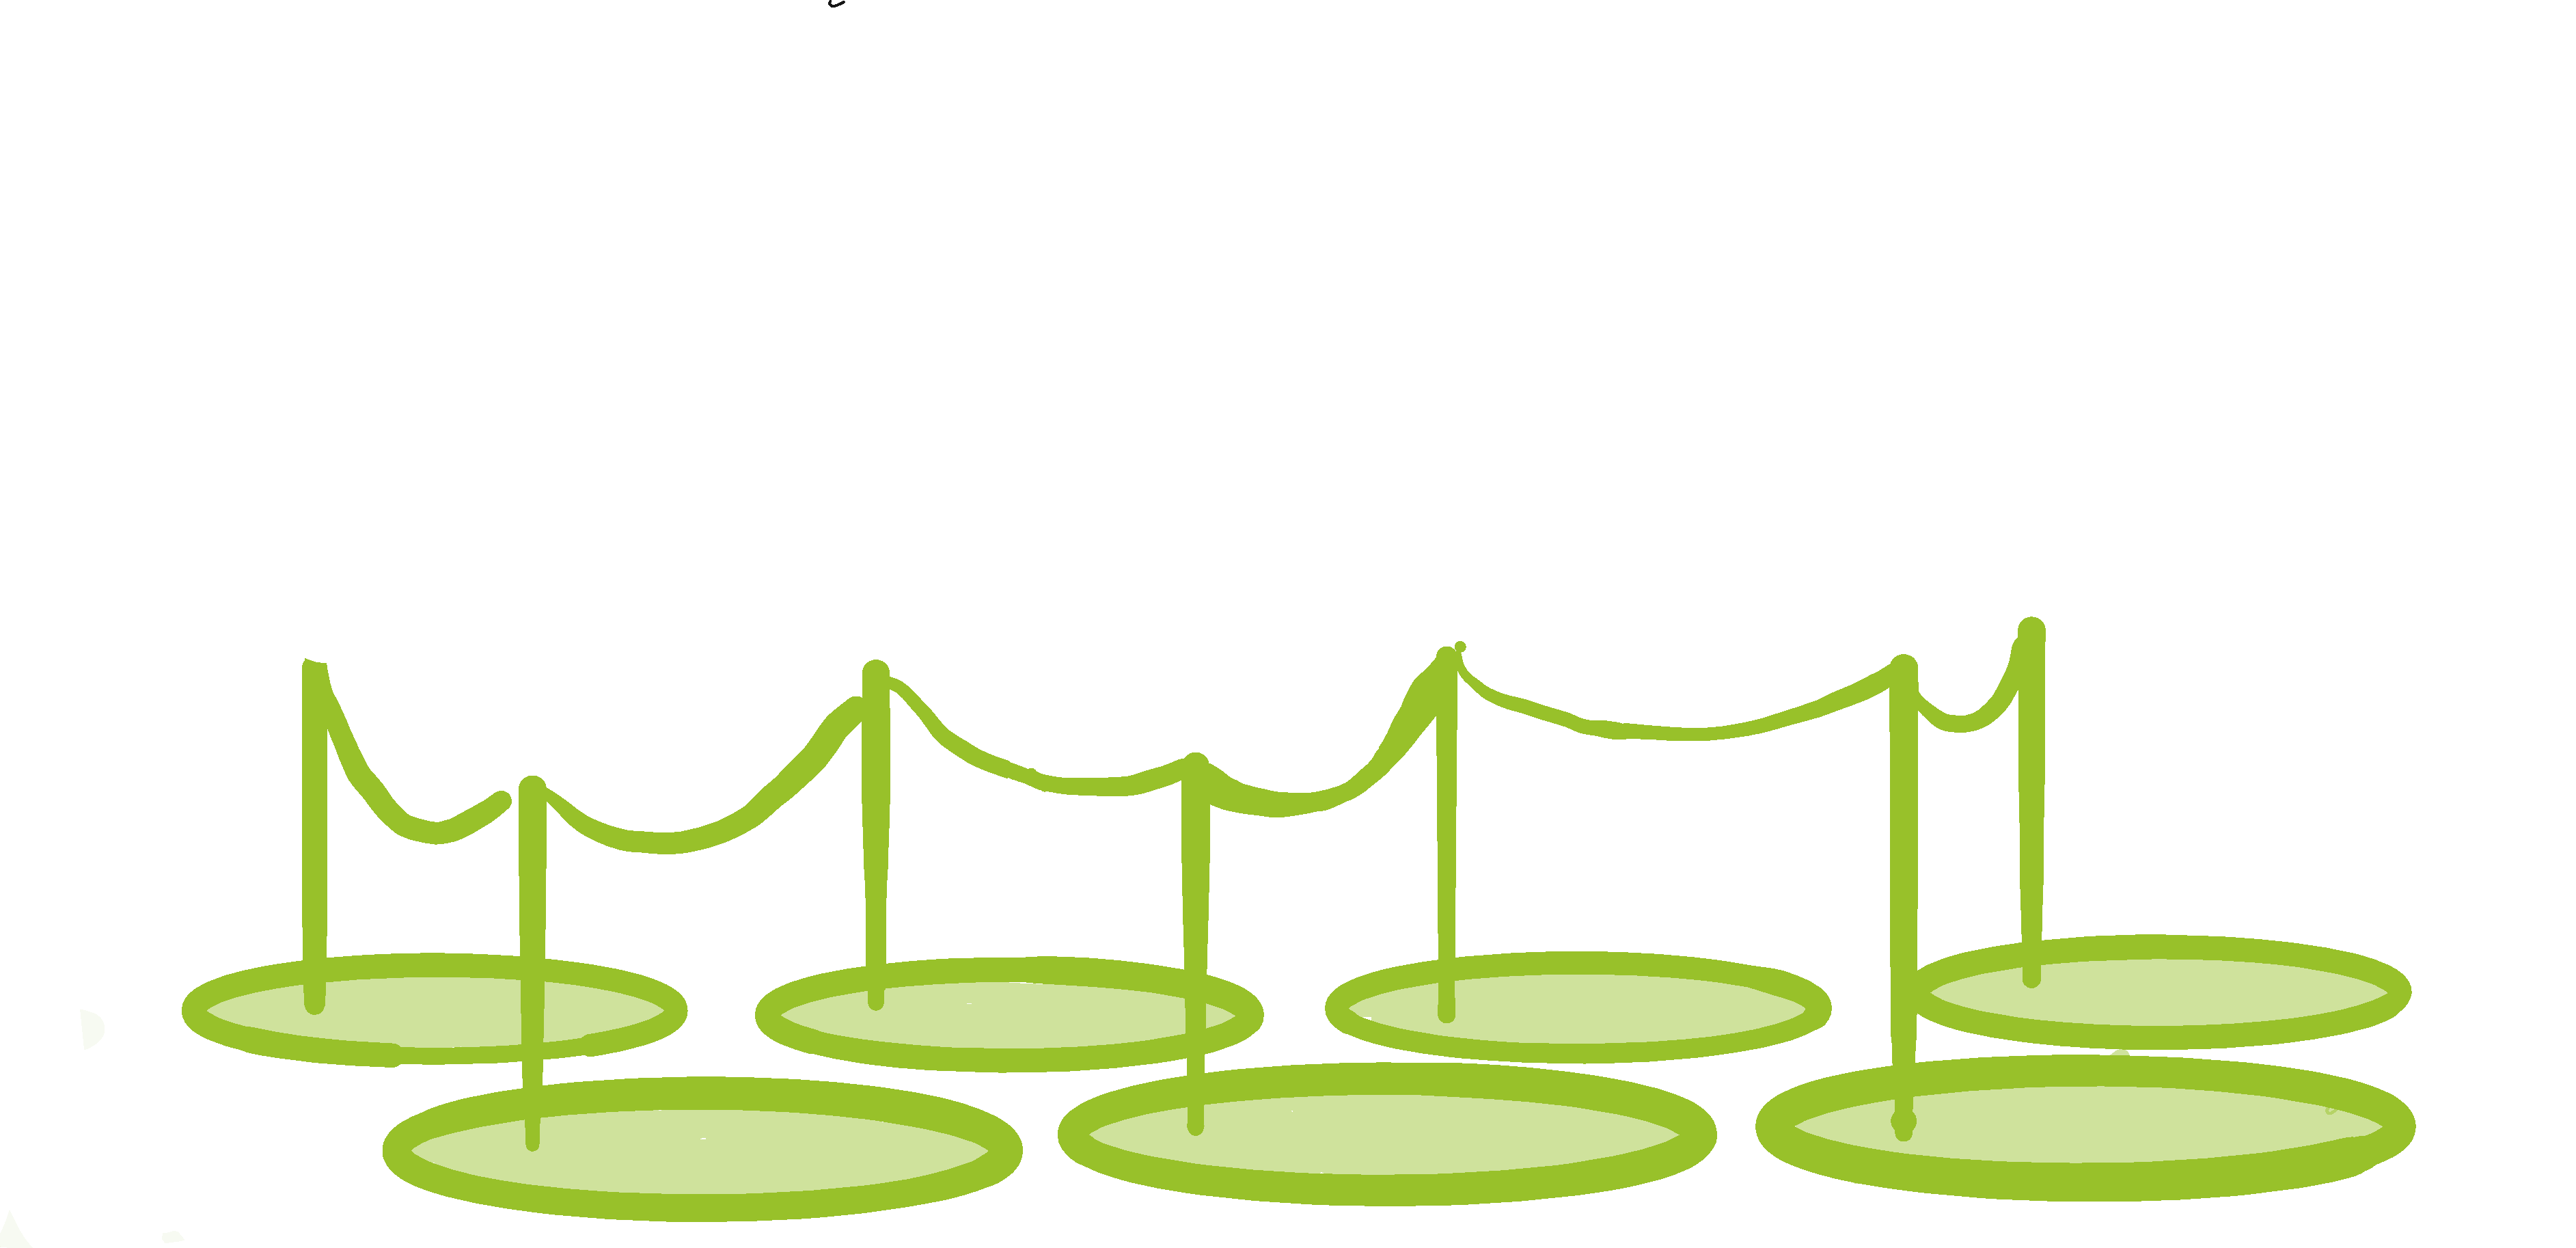
\includegraphics[width=\textwidth]{clump}
\end{column}
\begin{column}{0.07\textwidth}
{\Large$\underset{\phantom{?}}{\overset{\only<1,2>{?}\only<3>{\phantom{?}}}{
\includegraphics[width=\textwidth]{arrow}}}$}
\end{column}
\begin{column}{0.27\textwidth}
\centering
\only<1,2>{\Large ?} \only<3>{\Large \phantom{?}}
\includegraphics[width=\textwidth]<2>{clumps}
\includegraphics[width=\textwidth]<3>{clump_of_clumps}
\end{column}
\end{columns}
\vspace{1ex}
\begin{columns}
\begin{column}{0.05\textwidth}
\end{column}
\begin{column}{0.27\textwidth}
\centering
cell
\end{column}
\begin{column}{0.07\textwidth}
\end{column}
\begin{column}{0.27\textwidth}
\centering
clump
\end{column}
\begin{column}{0.07\textwidth}
\end{column}
\begin{column}{0.27\textwidth}
\centering
\only<3>{\phantom{(}}\only<1,2>{(}clump of clumps\only<1,2>{)}\only<3>{\phantom{)}}
\end{column}
\end{columns}
\vspace{2ex}
\caption{Analogy between (\subref{fig:natural}) natural and (\subref{fig:simulated}) simulated hierarchical fraternal transitions of individuality.}

\end{figure}


\end{frame}


\begin{frame}{Clumps \& Clumps of Clumps}
\begin{figure}
\begin{columns}
  \begin{column}{0.5\textwidth}
    \includegraphics<1>[width=\textwidth]{hsvmap/hsvmap-clump}%
    \includegraphics<2>[width=\textwidth]{hsvmap/hsvmap-clump}%
    \includegraphics<3>[width=\textwidth]{hsvmap/hsvmap-clumpofclumps}%
    \includegraphics<4>[width=\textwidth]{hsvmap/hsvmap-clumpsofclumps}%
  \end{column}
  \begin{column}{0.5\textwidth}
    \includegraphics<1>[width=\textwidth]{channelviz/channelviz-cell}%
    \includegraphics<2>[width=\textwidth]{channelviz/channelviz-clump}%
    \includegraphics<3>[width=\textwidth]{channelviz/channelviz-clumpofclumps}%
    \includegraphics<4>[width=\textwidth]{channelviz/channelviz-clumpsofclumps}%
  \end{column}
\end{columns}
\begin{columns}
  \begin{column}{0.5\textwidth}
    \begin{subfigure}[b]{\textwidth}
    \caption{channel ID HSV key}
    \end{subfigure}
  \end{column}
  \begin{column}{0.5\textwidth}
    \begin{subfigure}[b]{\textwidth}
    \caption{channel map visualization}
    \end{subfigure}
  \end{column}
\end{columns}
\caption{Visualization of hierarchically-nested signaling networks.}
\end{figure}
\end{frame}


\begin{frame}{Signals \& Resource}
  \begin{figure}
  \begin{columns}
  \begin{column}{0.02\textwidth}
  \rotatebox{90}{Level 2}
  \end{column}
  \begin{column}{0.49\textwidth}
      \centering
      \foreach \n in {1,...,12}{%
      \includegraphics<\n>[width=\textwidth,trim={0 0 0 250},clip]{big_res/frame-\n.png}%
      }%
  \end{column}
  \begin{column}{0.49\textwidth}
    \centering
    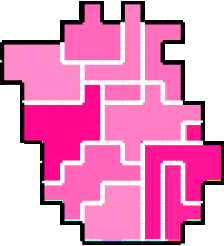
\includegraphics[width=0.4\textwidth]{channelviz/channelviz-clumpofclumps-crop.png}%
  \end{column}
  \end{columns}%
  \vspace{2ex}
  \begin{columns}
  \begin{column}{0.02\textwidth}
    \rotatebox{90}{Level 1}
  \end{column}
  \begin{column}{0.49\textwidth}
      \centering
      \foreach \n in {1,...,12}{%
      \includegraphics<\n>[width=\textwidth,trim={0 0 0 250},clip]{small_res/frame-\n.png}%
      }%
  \end{column}
  \begin{column}{0.49\textwidth}
    \centering
    \parbox{\widthof{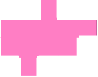
\includegraphics[width=0.2\textwidth]{channelviz/channelviz-clump-crop}}}{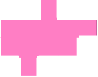
\includegraphics[width=0.2\textwidth]{channelviz/channelviz-clump-crop}}
    \textbf{~,~}
    \parbox{\widthof{
\includegraphics[width=0.2\textwidth]{channelviz/channelviz-clump2-crop}}}{
\includegraphics[width=0.2\textwidth]{channelviz/channelviz-clump2-crop}}
    \textbf{~,~\dots}
  \end{column}
  \end{columns}%
  \begin{columns}
  \begin{column}{0.02\textwidth}
  \end{column}
  \begin{column}{0.49\textwidth}
  \begin{subfigure}[b]{\textwidth}
  \caption{resource}
  \end{subfigure}
  \end{column}
  \begin{column}{0.49\textwidth}
  \begin{subfigure}[b]{\textwidth}
  \caption{same-channel networks}
  \end{subfigure}
  \end{column}
  \end{columns}
  \caption{Co-visualization of same-channel networks and resource distribution.}
  \end{figure}
\end{frame}

\begin{frame}{Multichannel Inheritance Outcomes}
  \begin{figure}
  \begin{subfigure}[b]{0.85\textwidth}
    \begin{columns}
    \begin{column}{0.05\textwidth}
      \caption{}~\\\vspace{0ex}~\\
      \label{fig:same_multichannel_offspring}
    \end{column}
    \begin{column}{0.95\textwidth}
      \colorbox{extralightgray}{
\includegraphics[width=\textwidth]{same_multichannel_offspring}}
  \end{column}
\end{columns}
  \end{subfigure}
  \begin{subfigure}[b]{0.85\textwidth}
      \begin{columns}
      \begin{column}{0.05\textwidth}
        \caption{}~\\\vspace{0ex}~\\
        \label{fig:new_lowchannel_offspring}
      \end{column}
      \begin{column}{0.95\textwidth}
        \colorbox{extralightgray}{
\includegraphics[width=\textwidth]{new_lowchannel_offspring}}
\end{column}
\end{columns}
  \end{subfigure}
  \begin{subfigure}[b]{0.85\textwidth}
      \begin{columns}
      \begin{column}{0.05\textwidth}
      \caption{}~\\\vspace{0ex}~\\
      \label{fig:new_highchannel_offspring}
      \end{column}
      \begin{column}{0.95\textwidth}
        \colorbox{extralightgray}{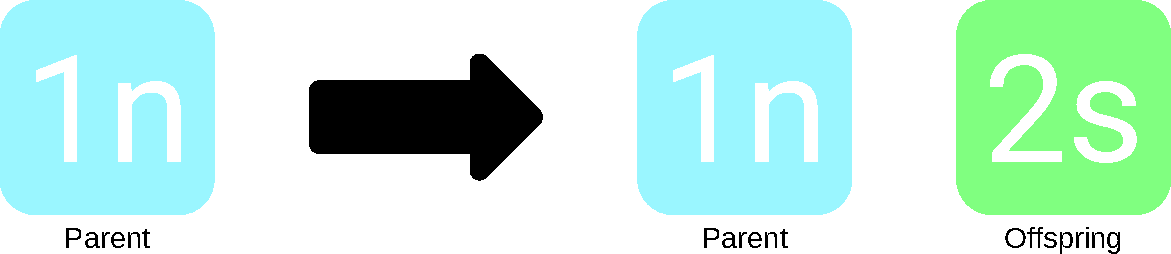
\includegraphics[width=\textwidth]{new_highchannel_offspring}\vspace{-10ex}}
\end{column}
\end{columns}
  \end{subfigure}
  \caption{
  Allowed multichannel inheritance outcomes;
  (\subref{fig:same_multichannel_offspring}) identical level 1 and 2 channels,
  (\subref{fig:new_lowchannel_offspring}) new level 1 channel with identical level 2 channel, and
  (\subref{fig:new_highchannel_offspring}) new level 1 and 2 channels.
  }
\end{figure}

\end{frame}

\begin{frame}{Signals \& Resource: Level 1 {\small(Clumps)} \& Level 2 {\small(Clumps of Clumps)}}%
  TODO how to explain that hierarchy enforced
\end{frame}
